\documentclass{beamer}
\usepackage{multicol}
\usepackage{natbib} 
\def\newblock{\hskip .11em plus .33em minus .07em}
\newcommand\independent{\protect\mathpalette{\protect\independenT}{\perp}} 
\def\independenT#1#2{\mathrel{\rlap{$#1#2$}\mkern2mu{#1#2}}} 
%\usepackage{beamerthemeBerkeley}
% Use either the one above or the one below
\usetheme{Pittsburgh}

\title{Sensitivity Analysis for Observational Studies}
%\author{	F. Daniel Hidalgo\\ }
%\date{\today}

\begin{document}

\frame{\titlepage}

%\section[Outline]{}
%\frame{\tableofcontents}

\begin{frame}
  \frametitle{Paul Rosenbaum}
  \begin{figure}[t]
    \centering
      
\includegraphics[scale=.8]{rosenbaum.jpg}
 \end{figure}
\end{frame}




\begin{frame}
  \frametitle{An Example}
  \begin{figure}[t]
  \centering
  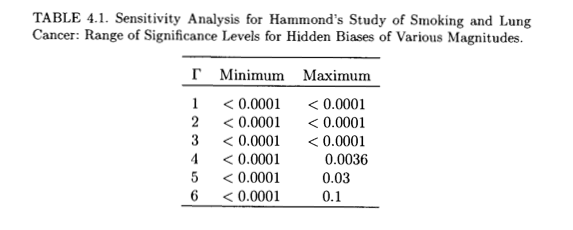
\includegraphics[scale=.6]{smoking_sensitivity.png}
\end{figure}
\end{frame}

\begin{frame}
  \frametitle{Another Example}
\begin{figure}[htbp]
	\centering
		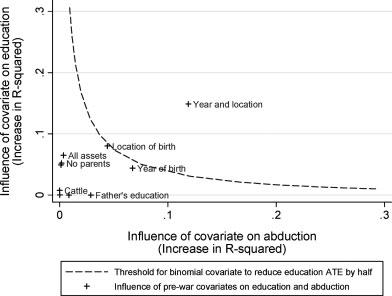
\includegraphics[height=3in]{blattman_sense.jpg}
	\label{fig:blattman_sense}
\end{figure}

\end{frame}


\begin{frame}[c]\frametitle{An Observational Study}
	\begin{table}
		\begin{center}
			\begin{tabular}{cccccccccc}
				$R_1$ & $R_2$ & $Z_1$ & $Z_2$ & $X_1$ & $X_2$ & $\pi_1$ & $\pi_2$ & $\frac{\pi_1}{\pi_1 + \pi_2}$ & $\Gamma $\\ \hline
				6 & 5 & 1 & 0 & 5 & 5 & .293 & .293 &  .5 &1 \\
				3 & 7 & 1 & 0 & 46 & 46 & .83 & .83 & .5 &1 \\
				4 & 7 & 1 & 0 & 3 & 3 & .2 & .2 &  .5 & 1\\
				7 & 14 & 1 & 0 & 25 &25 & .44 & .44 & .5& 1 \\

			\end{tabular}
		\end{center}
		\caption{Under the Naive Model}
	\end{table}
\end{frame}



\frame{
	\frametitle{Model of an Observational Study}
\begin{itemize}
\item<+-> $M$ units, each with an observed covariate vector $\mathbf{x}$.
Number the $M$ units $j=1,\dots,M$, so $\mathbf{x}_{[j]}$ and
$Z_{[j]}$ is the covariate and the treatment assignment for the $j$th
unit.
\item<+-> Unit $j$ is assigned to treatment with probability $\pi_j =
  \textrm{prob}(Z_{[j]}=1)$ and to control with probability $1-\pi_j =
  \textrm{prob}(Z_{[j]}=0)$
\item<+-> Treatments are assigned by flipping biased coins (each unit
  might have a different biased coin):
\[
\textrm{prob}(Z_{[1]}=z_1,\dots, Z_{[M]} =z_M) = \prod_{j=1}^M \pi_{[j]}^z\{1-\pi_{[j]}\}^{1-z_j}
\]
\end{itemize}
}


\begin{frame}
  \frametitle{Overt Bias}
  \begin{itemize}
  \item<+-> An observational study is free of \textit{hidden} bias if the
    $\pi$'s, though unknown, are known to only depend on the observed
    covariates, so two units with the same value of $\mathbf{x}$ have
    the same chance $\pi$ of receiving the treatment. 
\item<+-> The probability that $j$ will be in treatment is some unknown
  function of $\mathbf{x}$:  $\lambda(\mathbf{x}_{[j]})$, so the
  probability of treatment assignment becomes:
\[
\textrm{prob}(Z_{[1]}=z_1,\dots, Z_{[M]} =z_M) = \prod_{j=1}^M \lambda(\mathbf{x}_{[j]})^z\{1-\lambda(\mathbf{x}_{[j]})\}^{1-z_j}
\]
\item We are assuming \textbf{``randomization on the basis of a covariate''}.
  \end{itemize}
\end{frame}

%\begin{frame}
%  \frametitle{Matching on $\mathbf{x}$}
%  \begin{itemize}
%  \item<+-> From the $M$ units, select $N \leq M$ units and group them into
%    $S$ strata with $n_s$ units in stratum $s$.
%  \item<+-> Renumber the units so the $i$th unit in stratum $s$ has
%    treatment assignment $Z_{si}$ and covariate
%    $\mathbf{x_{si}}$. Write $\mathbf{Z}$ for
%    $(Z_{11},\dots,Z_{S,n_s}^T)$ and $m_s$ for the number of treated
%      units in stratum $s$; that is $m_s=\sum_i Z_{si}$, and
%      $\mathbf{m}=(m_1\dots,m_s)^T$.
%\item<+-> Stratification on $\mathbf{x}$ has strata that are homogenous
%  (or nearly so) in $x$, so two units are in the same strata only if
%  they have the same value of $\mathbf{x}$, that is
%  $\mathbf{x_{si}}=\mathbf{x_{sj}}$ for all $s$,$i$, and $j$. 
 % \end{itemize}
%\end{frame}


\begin{frame}
  \frametitle{Probability Distribution of $\mathbf{Z}|\mathbf{m}$}
\begin{itemize}
\item<+-> For inference, Rosenbaum proposes we use the conditional
  distribution of $\mathbf{Z}$ given $\mathbf{m}$.
\item<+-> For randomization inference, we want the full set of possibile
  treatment assignments ($\Omega$) and their associated
  probabilities. There are  $K=\prod_{s=1}^{S} \binom{n_s}{m_s}$
  possible assignments. 
\item<+-> Every treatment assignment $z \in \Omega$ has the
  same conditional probability: $\frac{1}{K}$, which means we can
  analyze the data as a uniform randomized experiment. 
\end{itemize}
\end{frame}

\begin{frame}
  \frametitle{A Model for Sensitivity Analysis}
  A sensitivity analysis asks: How would inferences about treatment
  effects be altered by hidden biases of various magnitudes?
\begin{itemize}
\item<+-> There is \emph{hidden} bias if two units with the same observed
  covariates \emph{x} have differing chances of receiving the
  treatment,  i.e. if $\mathbf{x}_{[j]} = \mathbf{x}_{[k]}$, but
  $\pi_{[j]} \neq \pi_{[k]}$ for some $j$ and $k$.
\item<+-> If units $j$ and $k$ are matched into pairs, the odds that units $j$ and
  $k$ receive the treatment are, respectively,
  $\pi_{[j]}/(1-\pi_{[j]})$ and $\pi_{[k]}/(1-\pi_{[k]})$, and the
  odds ratio is the ratio of these odds.
\item<+-> Conditional on the matching procedure, the probability of
  assignment to treatment: 
$$\textrm{P}(Z_{1}=1|Z_{s1}+Z_{s2}) = \frac{
    \pi_{s1}(1-\pi_{s2})}{\pi_{s1}(1-\pi_{s2}) + \pi_{s2}(1-\pi_{s1})} $$
\end{itemize}
\end{frame}

\begin{frame}
  \frametitle{$\Gamma$}
  \begin{itemize}
  \item<+-> The key parameter in a Rosenbaum-style sensitivity analysis is
    the treatment odds ratio, known as $\Gamma$.
  \item<+-> In a sensitivity analysis, we ask the effect of varying
    $\Gamma$ on our inferences, where $\Gamma$ is bounded as follows:
$$
\frac{1}{\Gamma} \leq
\frac{\pi_{[j]}(1-\pi_{[k]})}{\pi_{[k]}(1-\pi_{[j]})} \leq \Gamma
$$
\item<+-> A study is sensitive if values of $\Gamma$ close to 1 lead to
  inferences that are very different from those obtained assuming the
  study is free of hidden bias. 
  \end{itemize}
\end{frame}

\begin{frame}
  \frametitle{An Alternative Expression: Bias Due to an Unobserved Covariate}
  \begin{itemize}
  \item<+-> Unit $j$ has an observed covariate $\mathbf{x}_{[j]}$ and an
    unobserved covariate $u_{[j]}$. The model links the probability of
    assignment to treatment as follows:
$$\textrm{log}\left(\frac{\pi_{[j]}}{1- \pi_{[j]}} \right)=
k(\mathbf{x}_{[j]})+\gamma u_{[j]}$$ with $0\leq u_{[j]} \leq 1$ and
where $k(\cdot)$ is an unknown function and $\gamma$ is an unknown
parameter. 
\item<+-> After adjusting for $\mathbf{x}$, the odds ratio for two units
  in the same matched pair can be written as:
$$\frac{\pi_{[j]}(1-\pi_{[k]})}{\pi_{[k]}(1-\pi_{[j]})}  = \textrm{exp}\{\gamma(u_{[j]}-u_{[k]})\}  $$
  \end{itemize}
\end{frame}




\begin{frame}[c]\frametitle{Sensitivity of Significance Levels}
	
	\[
	\textrm{prob}(\mathbf{Z=z|m}) = \prod_{j=1}^M \left [\frac{e^{\gamma u_{s1}}}{e^{\gamma u_{s1}}+e^{\gamma u_{s2}}}\right ]^{z_{s1}} \left [\frac{e^{\gamma u_{s2}}}{e^{\gamma u_{s1}}+e^{\gamma u_{s2}}}\right ]^{1-z_{s1}} 
	\]
	
\end{frame}

\begin{frame}[c]\frametitle{An Observational Study}
	\begin{table}
		\begin{center}
			\begin{tabular}{cccccccccc}
				$R_1$ & $R_2$ & $Z_1$ & $Z_2$ & $X_1$ & $X_2$ & $U_1$ & $U_2$ & $\frac{\pi_1}{\pi_1 + \pi_2}$ & $\Gamma $\\ \hline
				6 & 5 & 1 & 0 & 5 & 5 & 1 & 0 &  .6667 &2 \\
				3 & 7 & 1 & 0 & 46 & 46 & 0 & 1 & .333 &2 \\
				4 & 7 & 1 & 0 & 3 & 3 & 0 & 0 &  .5 & 2\\
				7 & 14 & 1 & 0 & 25 &25 & 1 & 1 & .5 & 2 \\
			\end{tabular}
		\end{center}
		\caption{With an Omitted Variable}
	\end{table}
\end{frame}


\begin{frame}
  \frametitle{Sign-Score Statistics}
  \begin{itemize}
  \item<+-> General form of a Sign-Score test statistic:
$$ T=t(\mathbf{Z},\mathbf{r})= \sum_{s=1}^Sd_s\sum_{i=1}^2c_{si}Z_{si} $$
\item<+-> Wilcoxon signed rank statistic fo $S$ matched pairs is computed
  by ranking the absolute differences $|r_{s1}-r_{s2}| $ from 1 to $S$
  and summing the ranks of the pairs in which the treated unit had a
  higher response than the matched control. 
\item<+-> $d_s$ is the rank of $|r_{s1}-r_{s2}|$ with average ranks used
  for ties, and $c_{s1}=1$, $c_{s2}=0$ if $|r_{s1}>r_{r2}|$ with
  average ranks used for ties, and $c_{s1}=1$, $c_{s2}=0$ if
  $r_{s1}>r_{s2}$ or $c_{s1}=0$, $c_{s2}=1$ if $r_{s1}<r_{s2}$, and
  $c_{s1}=0$, $c_{s2}=0$ if  $r_{s1}=r_{s2}$ (pairs are tied). 
  \end{itemize}
  \end{frame}


\begin{frame}
  \frametitle{Sign Test}
  \begin{itemize}
  \item<+-> A particularly simple test for matched data is the sign test, which is simply the number of positive (or negative) within match differences
\item $d_s$ is 1 for all matched pairs, and $c_{s1}=1$, $c_{s2}=0$ if $r_{s1}>r_{r2}$. Similarly, $c_{s1}=0$, $c_{s2}=1$ if  $r_{s1}<r_{r2}$.
\item<+-> Exact p-values can be obtained using the binomial distribution.
  \end{itemize}
  \end{frame}

\begin{frame}[c]\frametitle{The Sign Test}
	\begin{table}
		\begin{center}
			\begin{tabular}{cccccccccc}
				$R_1$ & $R_2$ & $D$ & $C_1$ &$C_2$  & $U_1$ & $U_2$ & $\frac{\pi_1}{\pi_1 + \pi_2}$ & $\Gamma $\\ \hline
				6 & 5 & 1 & 1 & 0  & 1 & 0 &  .6667 &2 \\
				3 & 7 & 1 & 0 & 1  & 0 & 1 & .333 &2 \\
				4 & 7 & 1 & 0 & 1  & 0 & 0 &  .5 & 2\\
				7 & 14 & 1 & 0 & 1  & 1 & 1 & .5 & 2 \\
			\end{tabular}
		\end{center}
		\caption{With an Omitted Variable}
	\end{table}
	

\end{frame}

\begin{frame}[c]\frametitle{Unknowns}
	\begin{table}
		\begin{center}
			\begin{tabular}{cccccccccc}
				$R_1$ & $R_2$ & $D$ & $C_1$ &$C_2$  & $U_1$ & $U_2$ & $\frac{\pi_1}{\pi_1 + \pi_2}$ \\ \hline
				6 & 5 & 1 & 1 & 0  & ? & ? &  ?\\
				3 & 7 & 1 & 0 & 1  & ? & ? & ?  \\
				4 & 7 & 1 & 0 & 1  & ? & ? &  ?\\
				7 & 14 & 1 & 0 & 1  & ? & ? & ? \\
			\end{tabular}
		\end{center}
		\caption{With an Omitted Variable}
	\end{table}
\end{frame}




  \begin{frame}
    \frametitle{Inference}
    \begin{itemize}
    \item In a randomized experiment, $t(\mathbf{Z},\mathbf{r})$ is
      compared to the randomization distribution under the null
      hypothesis. In effect, $t(\mathbf{Z},\mathbf{r})$ is the sum of
      $S$ independent random variables where the $s$th variable equals
      $d_s$ with probability $1/2$.
    \item If there is hidden bias, we don't know what the
      randomization distribution is under the null hypothesis! But we
      can still \textbf{bound} the possible distributions under a
      given amount of possible hidden bias.
\end{itemize}
  \end{frame}

\begin{frame}[c]\frametitle{Inference with an Unknown Confounder}
	\begin{itemize}
		\item<+-> For each possible $(\gamma, \mathbf{u})$, the statistic $t(\mathbf{Z,r})$ is the sum of $S$ independent random variables, where the $s$th variable equals $d_s$ with probability 
		\[
		p_s = \frac{c_{s1}\textrm{exp}(\gamma u_{s1}) + c_{s2}\textrm{exp}(\gamma u_{s2})}{\textrm{exp}(\gamma u_{s1}) + \textrm{exp}(\gamma u_{s2})}
		\]
		\item<+-> With $\Gamma = exp(\gamma)$ define $p^{+}_s$ and $p_s^-$ in the following way:
      \begin{eqnarray}
        \label{eq:1}
        p_s^+=\frac{\Gamma}{1+\Gamma} \\
        p_s^-=\frac{1}{1+\Gamma} 
     \end{eqnarray}

	\end{itemize}
\end{frame}

\begin{frame}[c]\frametitle{Assume the worse case scenario}
	\begin{table}
		\begin{center}
			\begin{tabular}{cccccccccc}
				$R_1$ & $R_2$ & $D$ & $C_1$ &$C_2$  & $U_1$ & $U_2$ & $\frac{\pi_1}{\pi_1 + \pi_2}$ \\ \hline
				6 & 5 & 1 & 1 & 0  & 1 & 0 &  ?\\
				3 & 7 & 1 & 0 & 1  & 0 & 1 & ?  \\
				4 & 7 & 1 & 0 & 1  & 0 & 1 &  ?\\
				7 & 14 & 1 & 0 & 1  & 0 & 1 & ? \\
			\end{tabular}
		\end{center}
		\caption{With an Omitted Variable}
	\end{table}
\end{frame}


\begin{frame}[c]\frametitle{Choose a $\Gamma$}
	\begin{table}
		\begin{center}
			\begin{tabular}{cccccccccc}
				$R_1$ & $R_2$ & $D$ & $C_1$ &$C_2$  & $U_1$ & $U_2$ & $\frac{\pi_1}{\pi_1 + \pi_2}$ & $\Gamma$\\ \hline
				6 & 5 & 1 & 1 & 0  & 1 & 0 &  .33 & 2\\
				3 & 7 & 1 & 0 & 1  & 0 & 1 & .66  & 2\\
				4 & 7 & 1 & 0 & 1  & 0 & 1 &  .66 & 2\\
				7 & 14 & 1 & 0 & 1  & 0 & 1 & .66 & 2\\
			\end{tabular}
		\end{center}
		\caption{With an Omitted Variable}
	\end{table}
\end{frame}


\begin{frame}[c]\frametitle{Choose another $\Gamma$}
	\begin{table}
		\begin{center}
			\begin{tabular}{cccccccccc}
				$R_1$ & $R_2$ & $D$ & $C_1$ &$C_2$  & $U_1$ & $U_2$ & $\frac{\pi_1}{\pi_1 + \pi_2}$ & $\Gamma$\\ \hline
				6 & 5 & 1 & 1 & 0  & 1 & 0 &  .2 & 4\\
				3 & 7 & 1 & 0 & 1  & 0 & 1 & .8  & 4\\
				4 & 7 & 1 & 0 & 1  & 0 & 1 &  .8 & 4\\
				7 & 14 & 1 & 0 & 1  & 0 & 1 & .8 & 4\\
			\end{tabular}
		\end{center}
		\caption{With an Omitted Variable}
	\end{table}
\end{frame}



  \begin{frame}
    \frametitle{Bounds}
    \begin{itemize}
    \item Define $T^+$ to be the sum of $S$ independent random
      variables, where the $s$th variable takes the value of $d_s$
      with probability $p^+_s$ and takes the value of 0 with
      probability $1-p^+_s$. Define $T^-$ similarly with $p^-_s$
   \item If the treatment has no effect, then for each fixed $\gamma \geq 0$,
$$\textrm{prob}(T^+\geq a) \geq \textrm{prob}\{T>a|\mathbf{m}\} \geq
\textrm{prob}(T^- \geq a)$$
for all $a$ and $\mathbf{u} \in U$.
  \end{itemize}
  \end{frame}
  \begin{frame}
    \frametitle{More on Bounds}
What do these bounds actually mean?

    \begin{itemize}
   \item<+-> The upper bound $\textrm{prob}(T^+\geq a) $ is the
      distribution of $t(\mathbf{Z},\mathbf{r})$ when $u_{si}=c_{si}$
      and the lower bound $\textrm{prob}(T^- \geq a)$ is the
      distribution when $u_{si}=1-c_{si}$
    \item<+-> This means that the bounds are attained values of
      $\mathbf{u}$ that exhibit a strong, near perfect, relationship
      with $\mathbf{r}$, as $c_{si}$ is a function of $r_{si}$. 
    \end{itemize}
  \end{frame}
  \begin{frame}
    \frametitle{Calculating P-Values}
    \begin{itemize}
    \item<+-> The \textrm{exact} P-values can be calculated, but not practical in
      moderate or larger datasets.
    \item<+-> Large sample approximations using: 
$$E(T^+)=\sum_{s=1}^Sd_sp^+_s$$
$$\textrm{var}(T^+)=\sum_{s=1}^Sd^2_sp^+_s(1-p^+_s)$$

    \end{itemize}
  \end{frame}


\begin{frame}[c]\frametitle{Amplification}
	\begin{itemize}
		\item<+-> 	What if we believe that a confounder exists but it's not perfectly correlated with the outcome? 
		\item<+-> An amplification allows the researcher to ask, how would my inferences change under different correlations between $u$ and $r$, as well as $u$ and $r$?
		\item<+-> 3 unknowns:
		\begin{enumerate}
			\item<+-> $\Delta$ is degree of association between $u$ and $r$
			\item<+-> $\Lambda$ is degree of association between $u$ and $Z$
			\item<+-> $\Gamma$ is degree of association between $u$ and $Z$ when $u$ is perfectly correlated with $Z$.   
		\end{enumerate}
		\item<+-> $\Gamma$ can be decomposed as follows:
		$$\Gamma = \frac{\Delta \Lambda + 1}{\Delta + \Lambda}$$
	\end{itemize}
 
	
\end{frame}


\end{document}
